\documentclass[10pt,firamath,cours]{nsi}
\begin{document}
\setcounter{chapter}{13}


\chapter{Gestion des processus et ressources}


\section{Systèmes d'exploitation multitâches}
De nos jour les OS permettent d'exécuter plusieurs programmes en même temps :\\

\begin{itemize}
	\item jouer à un jeu vidéo ;
    \item parler avec ses amis sur Discord ;
    \item utiliser un logiciel de streaming de type OBS ;
    \item et d'autres choses encore...
\end{itemize}
Lorsqu'on ouvre le gestionnaire des tâches de \textsc{Windows}, voici ce qu'on obtient

{Gestionnaire des tâches \textsc{Windows}}
\begin{center}
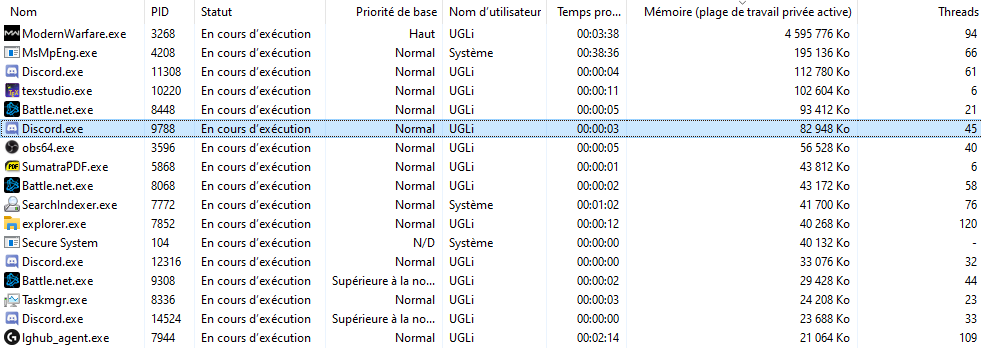
\includegraphics[width=\linewidth]{img/gest}\\
\small \textit{Une partie des tâches en cours sur mon ordinateur;}
\end{center}


Peu importe le nombre de c\oe urs du CPU, la multitude des programmes en cours d'exécution montre que l'OS dispose d'un système pour gérer ces exécutions simultanées.\\
Puisque tous les programmes ne peuvent « tourner en même temps» on parle d'\textit{exécution concurrente}.

\section{Les processus}
\subsection{Exécution d'un programme seul (version théorique et simplifiée)}
Un \textit{exécutable} est un fichier qui contient des instructions en langage machine.\\
Lors de son ouverture
\begin{itemize}
	\item l'OS charge le programme dans la RAM, à une certaine adresse-mémoire ;
    \item il écrit cette adresse dans le registre PC (\textit{program counter}) du CPU.
\end{itemize}
À chaque cycle d'horloge, le CPU lit l'instruction à l'adresse courante, l'exécute, puis passe à l'instruction suivante jusqu'à la dernière.


\subsection{En réalité}
Dans le modèle précédent, un seul programme peut être lancé et l'OS doit attendre qu'il « rende la main» pour continuer.\\

Il n'est pas possible de lancer 2 programmes ou plus en même temps, on a affaire à un OS \textit{monotâche}... Or nos OS actuels sont clairement multitâches.

\subsection{Multitâche coopératif}
Il consiste à laisser les programmes décider du moment où ils doivent rendre la main aux autres. Celui-ci pose cependant deux principales difficultés :
\begin{itemize}
	\item il faut que le multitâche soit pris en compte lors de l'écriture des programmes ;
    \item en cas d'erreur le système tout entier peut se retrouver bloqué.
\end{itemize}
C'est ce type de multitâche que l'on retrouve dans \textsc{Windows 3.1} (1993) ou \textsc{Mac OS 9} (1999).\\
\begin{center}

\includegraphics[height=2cm]{img/win31}\hspace{2cm}
\includegraphics[height=2cm]{img/macos}
\end{center}

\subsection{Multitâche préemptif}
Il consiste à octroyer un certain temps d'exécution au programme avant de reprendre la main de force en sauvegardant l'état du processus, au moyen d'une interruption programmable.\\
Ce type de multitâche se retrouve dans les systèmes d'exploitation Unix (1969) et aussi dans les systèmes plus grand-public depuis Windows 95 (1995) et Mac OS X (2001).\\

C'est sur la 2\eme approche que nous allons nous concentrer.

\subsection{Interruption}
C'est un signal envoyé au CPU lorsqu'un évènement se produit : un disque dur a terminé d'écrire des octets, un clavier signale qu'une touche est pressée, \textit{et c\ae tera}.\\

Lors d'une interruption, le CPU arrête l'exécution du programme en cours.\\
Celle-ci est communiquée à un programme appelé \textit{gestionnaire d'interruptions}, accompagnée d'une copie de l'ensemble des valeurs des registres du CPU.\\
En fonction de l'interruption, le gestionnaire passe la main à un autre programme.

    
\subsection{Les interruptions d'horloge}
Le CPU génère de lui-même des interruptions à intervalles de temps fixe.\\
De nos jours un CPU moderne les génère à une fréquence de 10 MHz, donc toutes les 100 nanosecondes (un dix-millième de milliseconde).\\

Ce sont elles qui permettent d'exécuter les programmes de manière concurrente.


\begin{definition}[ : exécutable]
    Fichier binaire contenant des instructions en langage-machine directement exécutables par le CPU.    
\end{definition}
    
\begin{definition}[ : processus]
    Un des programmes en cours d'exécution. En général il est décrit par
    \begin{itemize}
        \item un \textit{identifiant} unique;
        \item son \textit{état} (effectivement en cours d'exécution, en attente ...);
        \item la \textit{mémoire} allouée par l'OS au programme;
        \item les \textit{ressources} utilisées par le programme (fichiers, connexions réseaux, matériels \textit{et c\ae tera});
        \item les \textit{valeurs des registres} du CPU.
    \end{itemize}        
\end{definition}

\begin{definition}[ : PCB]
    Pour chaque processus, l'OS stocke sa description dans une structure de données appelée \textit{PCB}, pour \textit{Process Control Bloc}.    
\end{definition}

\begin{definition}[ : exécution concurrente]
    Deux processus s'exécutent de manière concurrente si les intervalles de temps entre le début et la fin de leur exécution ont une partie commune.    
\end{definition}

On ne parlera pas d'exécution \textit{parallèle} (lorsque deux processus s'effectuent \textit{réellement} en même temps).


\subsection{Arborescence des processus}
En général (c'est le cas avec les OS de type \textsc{UNIX}), l'OS crée au démarrage un processus de base qui à son tour va créer d'autres processus, appelés \textit{processus fils}, et ainsi de suite.\\

Cela donne lieu à une \textit{arborescence de processus}.


\subsection{Processus légers ou thread}
Les \textit{threads} sont des processus particuliers crées par des processus qui se veulent eux-mêmes multitâches.\\
La principale différence entre thread et processus est que contrairement aux processus qui \textit{a priori} sont isolés les uns des autres, les threads \textit{partagent des variables globales}.\\
La commutation de contexte entre threads (voir plus loin) est également plus rapide qu'entre processus.\\



\section{L'ordonnanceur}


C'est le composant de l'OS chargé de \textit{choisir l'ordre d'exécution} des différents processus.\\
De son point de vue les threads sont des processus à part entière.

\begin{exemple}[ de fonctionnement]
    \begin{enumerate}
        \item un processus p1 est en cours d'utilisation ;
        \item une interruption d'horloge survient ;
        \item le \textit{gestionnaire d'interruption} (GI) est appelé et sauvegarde l'état des registres du CPU à un endroit particulier de la mémoire ;
        \item il fait appel à l'\textit{ordonnanceur} qui \textit{décide} à quel autre processus p2  il veut passer la main ;
        \item le GI restaure les valeurs des registres du CPU qui on été sauvegardées la dernière fois que p2 a été interrompu ;
        \item le GI rend la main : p2 reprend.
    \end{enumerate}
    Les phases \textbf{2.} à \textbf{5.} s'appellent une \textit{commutation de contexte}.        
\end{exemple}

\subsection{\'Etats d'un processus}
Un processus peut parfois être de lui-même en pause (\mintinline{python}{sleep} en Python).\\
De même il peut être en attente d'une ressource : par exemple lors de l'appel de \mintinline{python}{input}, le programme sollicite le clavier et attend une réponse.\\
Parfois aussi, des erreurs peuvent se produire (programme mal codé, problème matériel...).\\

Toutes ces conditions amènent l'OS à définir l'\textit{état} de chaque processus.


\begin{encadrecolore}{Les différents états}{UGLiPurple}
    \begin{itemize}
        \item \textbf{Nouveau : } état éphémère : l'OS vient de copier l'exécutable en mémoire et créé son PCB ; 
        \item \textbf{Prêt : } le processus est dans l'ensemble des processus qui peuvent être choisis par l'ordonnanceur pour être exécutés : il attend son tour ;
        \item \textbf{En exécution :} le processus est effectivement en train de s'exécuter ;
        \item \textbf{En attente :} le processus est interrompu et est en attente d'un évènement externe : qu'une allocation mémoire soit effectuée, qu'une E/S soit activée, qu'un des périphériques dont il a besoin soit libre...
        \item \textbf{Terminé :} état éphémère : l'OS va libérer la mémoire allouée au processus ainsi que les ressources qu'il utilise et effacer son PCB.
    \end{itemize}
    À tout moment une erreur peut conduire à la terminaison du processus.        
\end{encadrecolore}

\subsection{Cycle de vie d'un processus}
\begin{center}
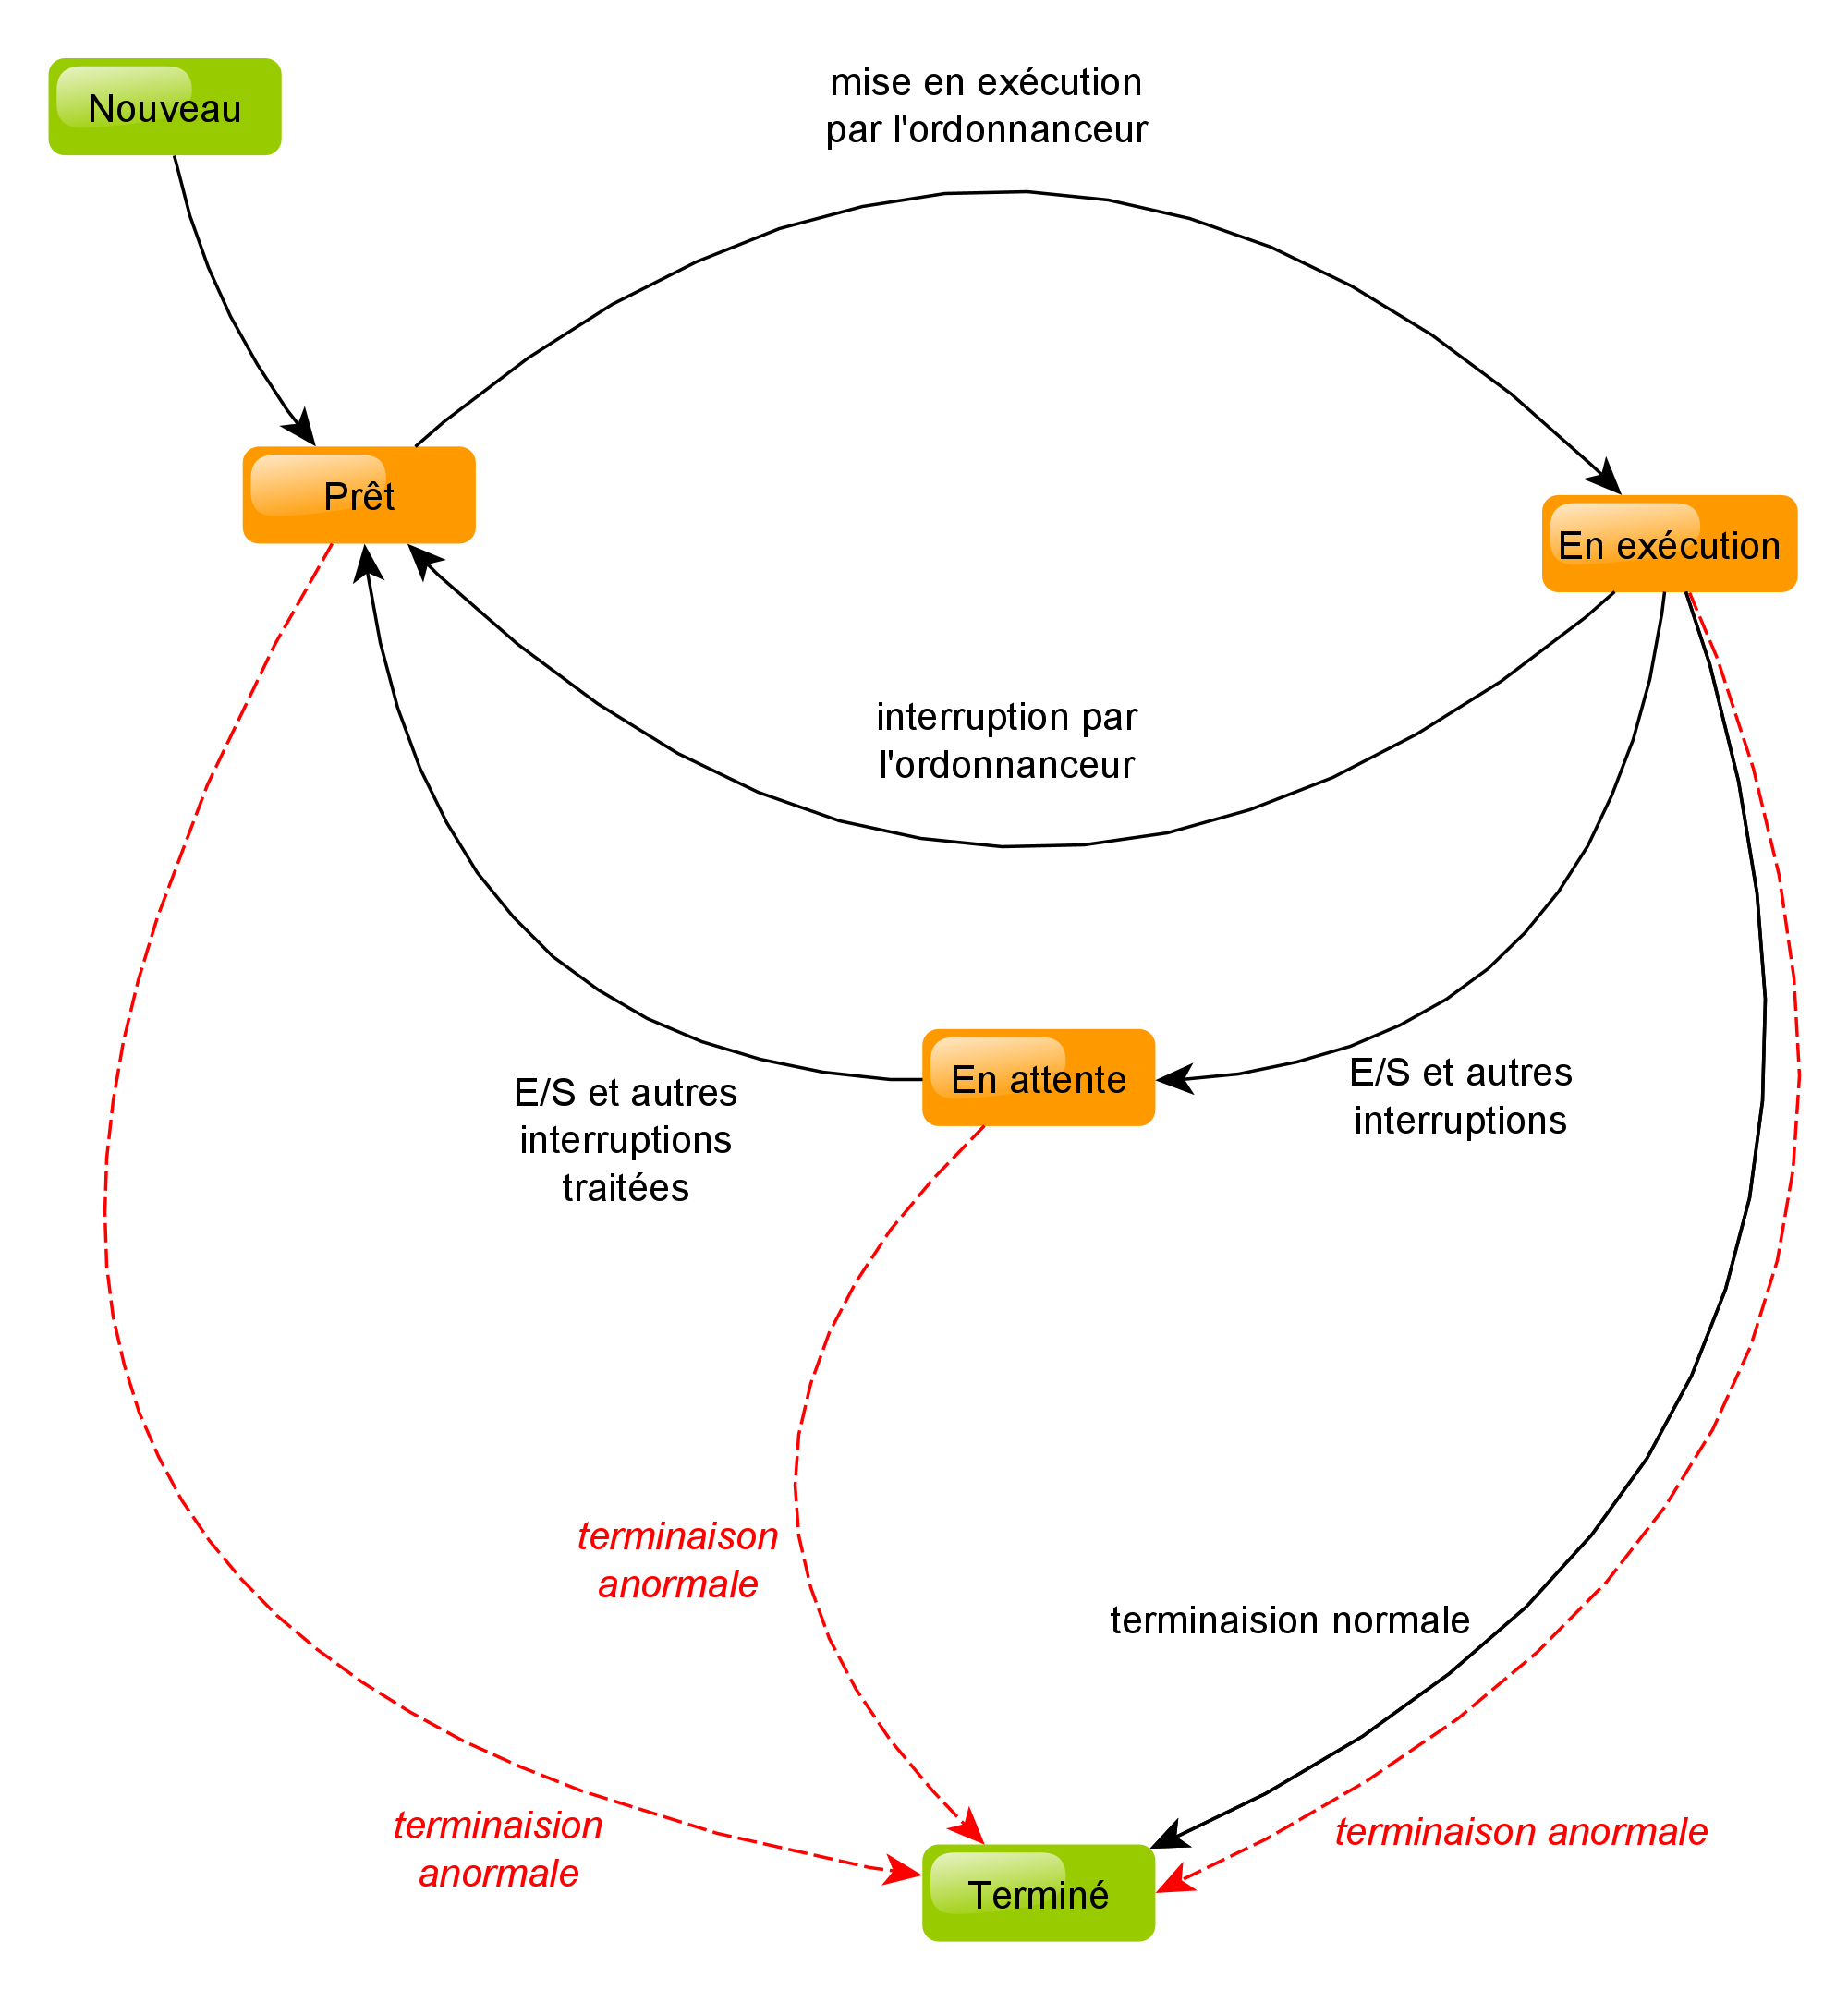
\includegraphics[width=10cm]{img/cycle_proc}
\end{center}


\section{Les stratégies d'ordonnancement}

\subsection{Quel algorithme utiliser ?}
\begin{center}
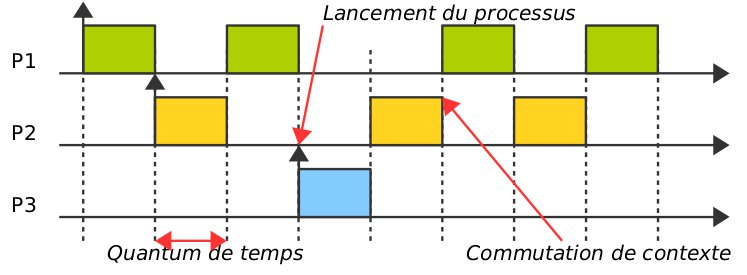
\includegraphics[width=9cm]{img/3proc}
\end{center}
On observe ici le déroulement \textit{pseudo-parallèle} de 3 processus.
\begin{itemize}
	\item P1 débute à $t=0$, utilise 4 quanta, sur une durée de 8 quanta ;
    \item P2 débute à $t=1$, utilise 3 quanta, sur une durée de 6 quanta ;
    \item P3 débute à $t=3$, utilise 1 quantum, sur une durée de 1 quantum.
\end{itemize}

\begin{encadrecolore}{Différents algorithmes}{UGLiGreen}
    \begin{itemize}
        \item \textbf{FIFO} : les processus sont placés dans une file et exécutés dans cet ordre, puis remis dans la file
        \item \textbf{SJF} : (\textit{Shortest Job First}) le processus le plus court est exécuté en premier
        \item \textbf{Round Robin} : Chaque processus aura la main pendant un certain temps, le même pour tous
    \end{itemize}        
\end{encadrecolore}

\begin{encadrecolore}{Priorité}{UGLiYellow}
Il est possible d'attacher une priorité à chaque processus de sorte que
\begin{itemize}
	\item les processus importants soient exécutés en premier ou plus souvent que les autres ;
    \item les processus peu importants ne soient exécutés que quand le CPU n'est pas beaucoup sollicité.
\end{itemize}
\end{encadrecolore}

La plupart des OS multitâches actuels utilisent (pour partie) une combinaison des algorithmes précédents combinés avec des priorités.\\
Dans les systèmes \textsc{UNIX}, la priorité d'un processus s'appelle \textit{niceness}.


\subsection{Exemples détaillés}
On considère les processus suivants
\begin{center}
    \tabstyle[UGLiOrange]
\begin{tabular}{|c|c|c|c|}
\ccell Processus & \ccell Départ & \ccell Durée & \ccell Priorité \\
\hline
P1 & 0 & 4 & basse \\
\hline
P2 & 3 & 7 & basse \\
\hline
P3 & 7 & 3 & haute \\
\hline
P4 & 9 & 2 & haute \\
\hline
\end{tabular}
\end{center}

\subsubsection{FIFO sans priorités}
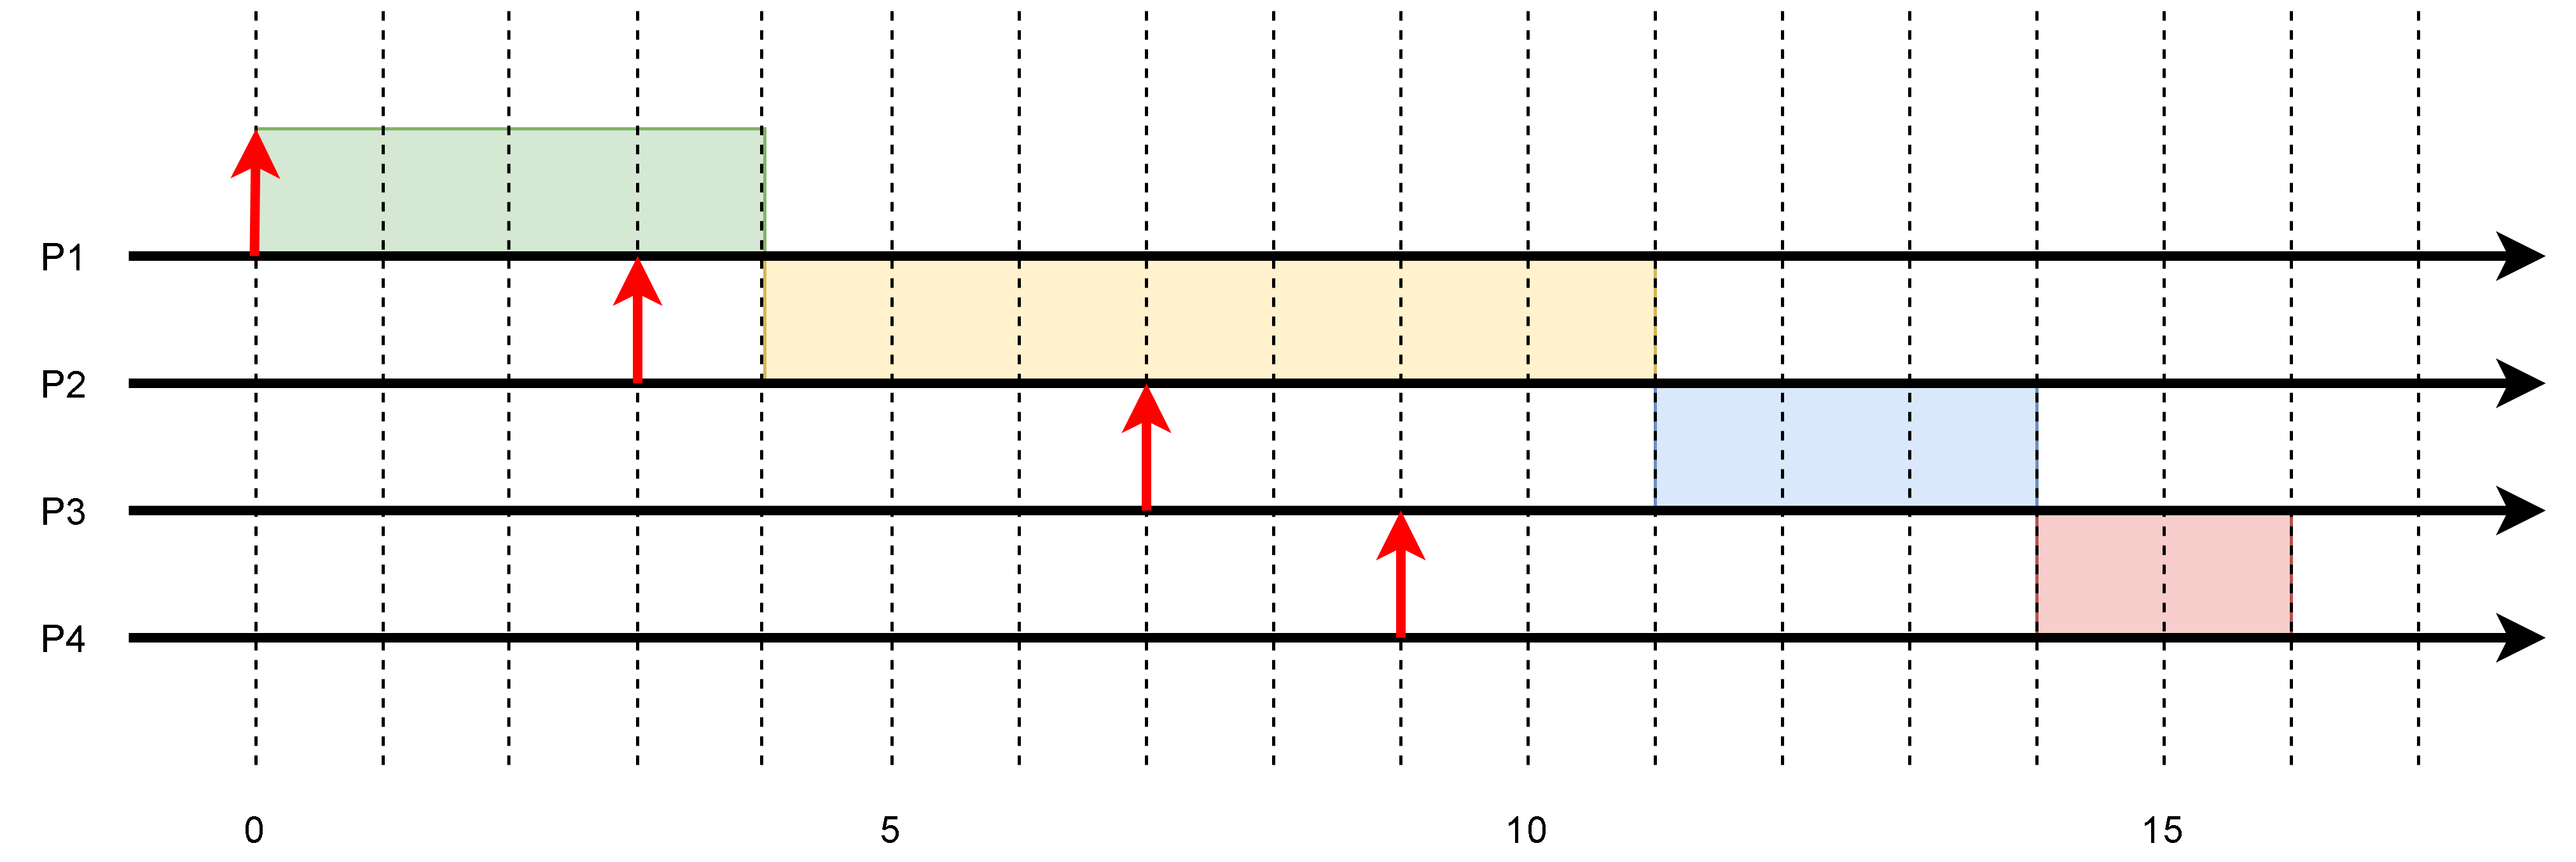
\includegraphics[width=\linewidth]{img/FIFO}

\subsubsection{FIFO avec priorités}
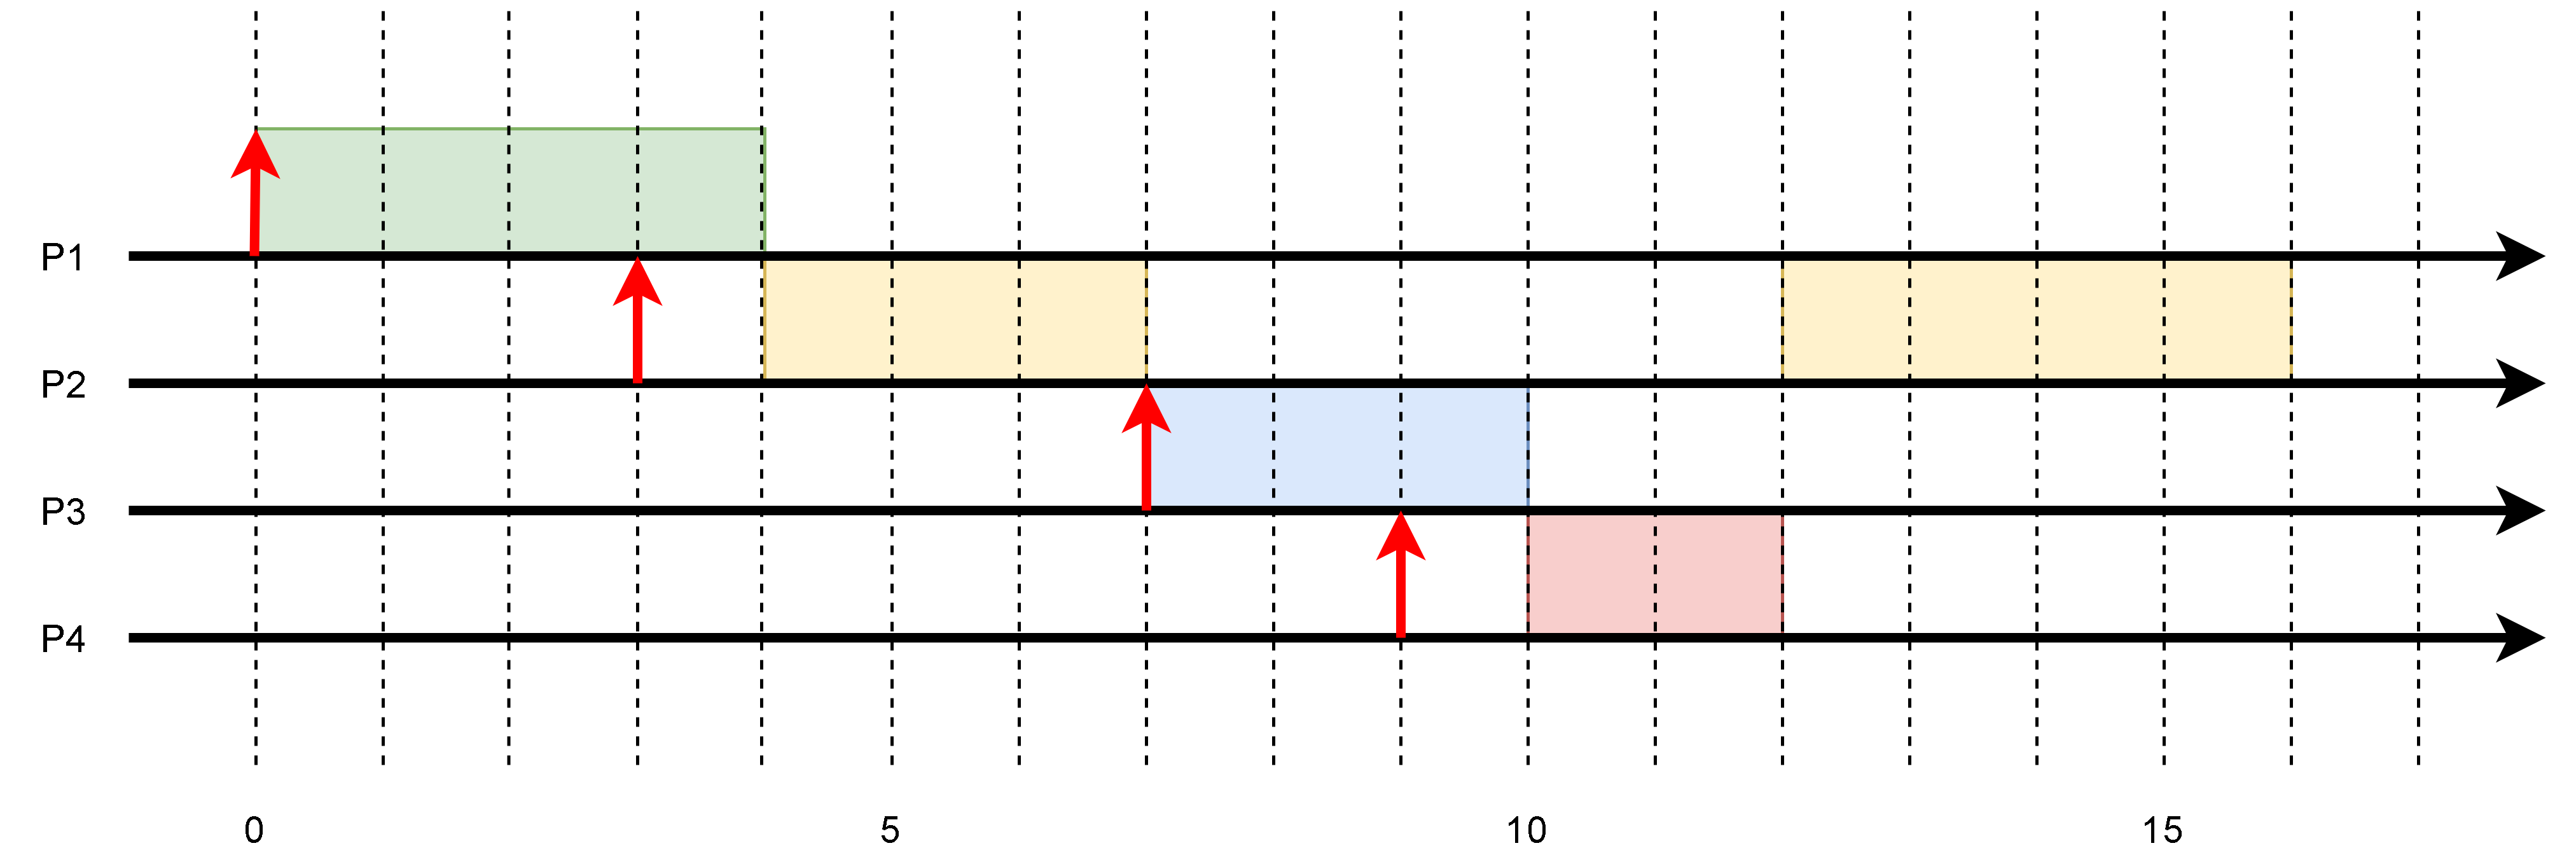
\includegraphics[width=\linewidth]{img/FIFOP}

\subsubsection{Round Robin sans priorités}
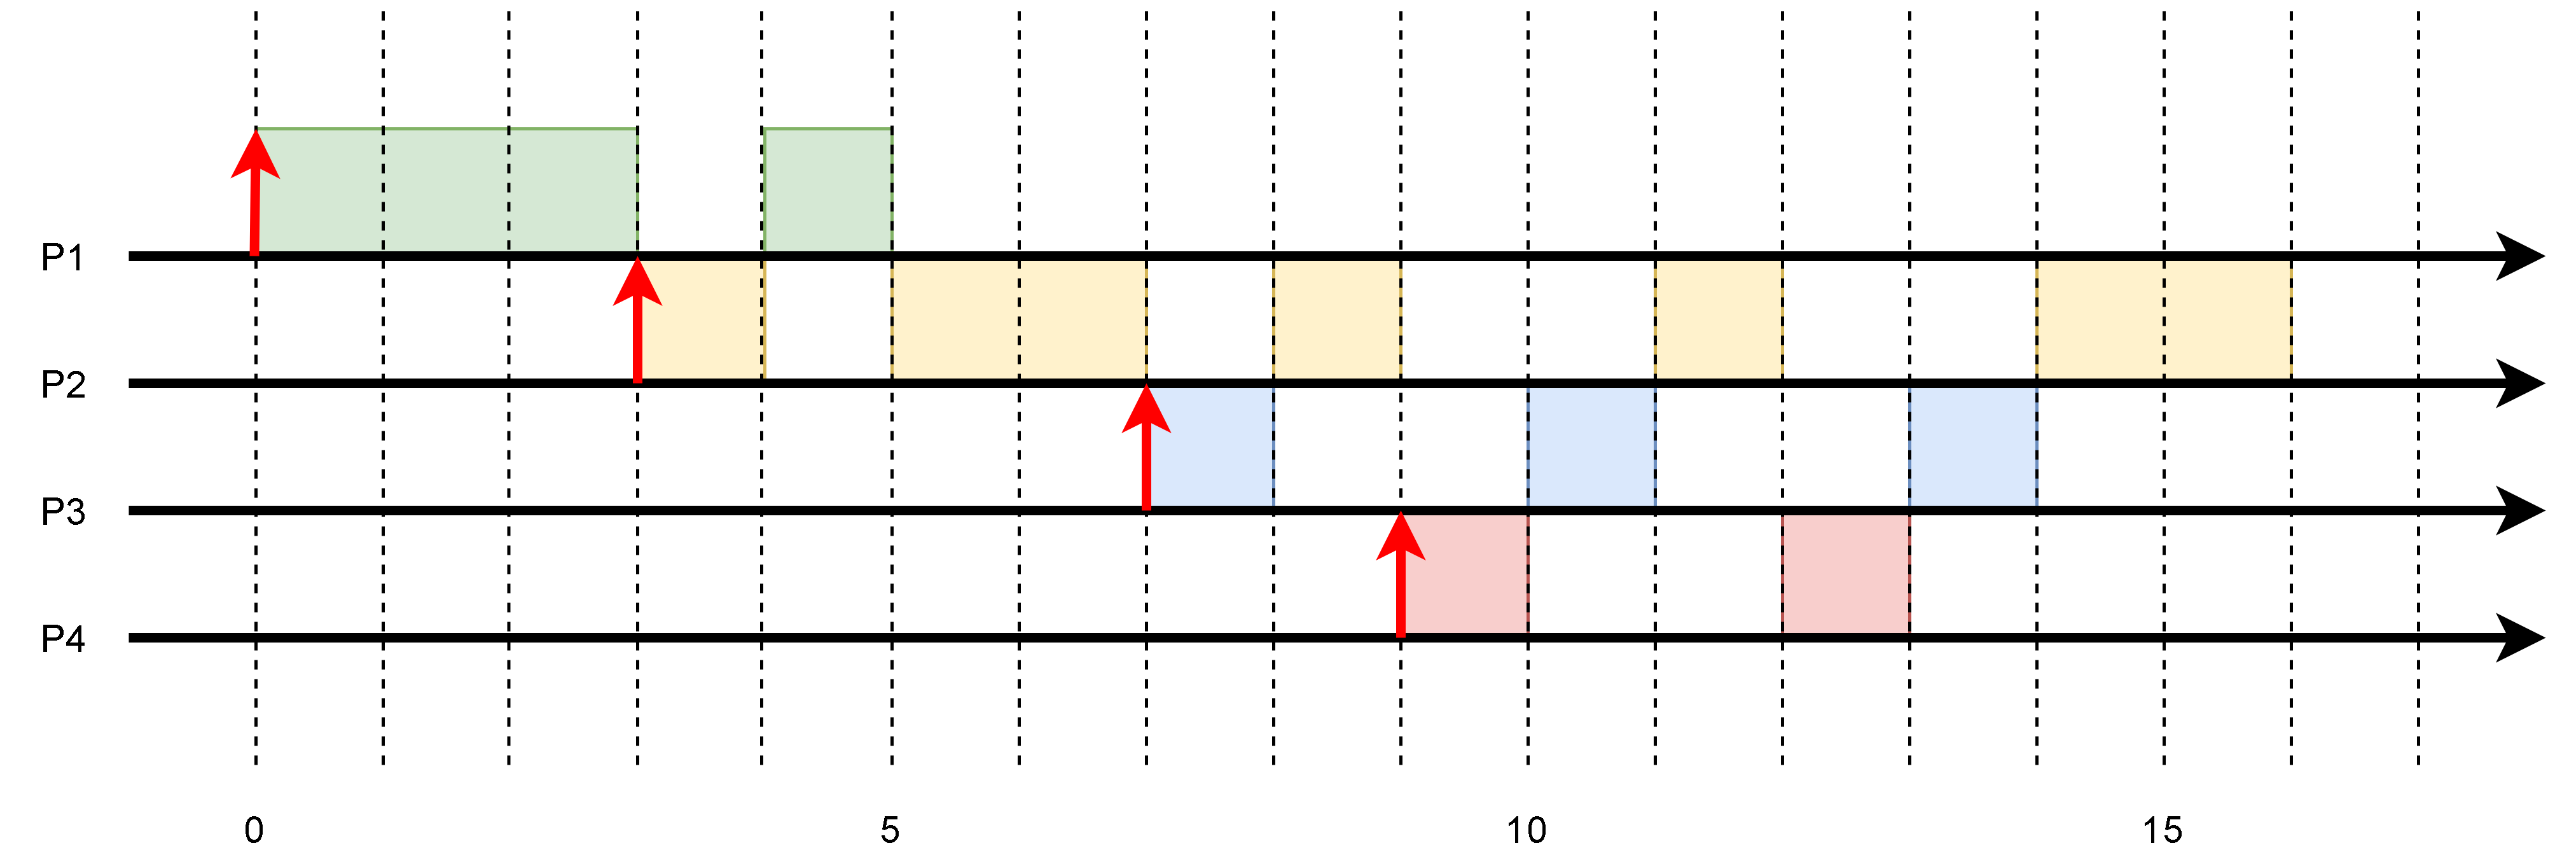
\includegraphics[width=\linewidth]{img/RR}

\subsubsection{Round Robin avec priorités}
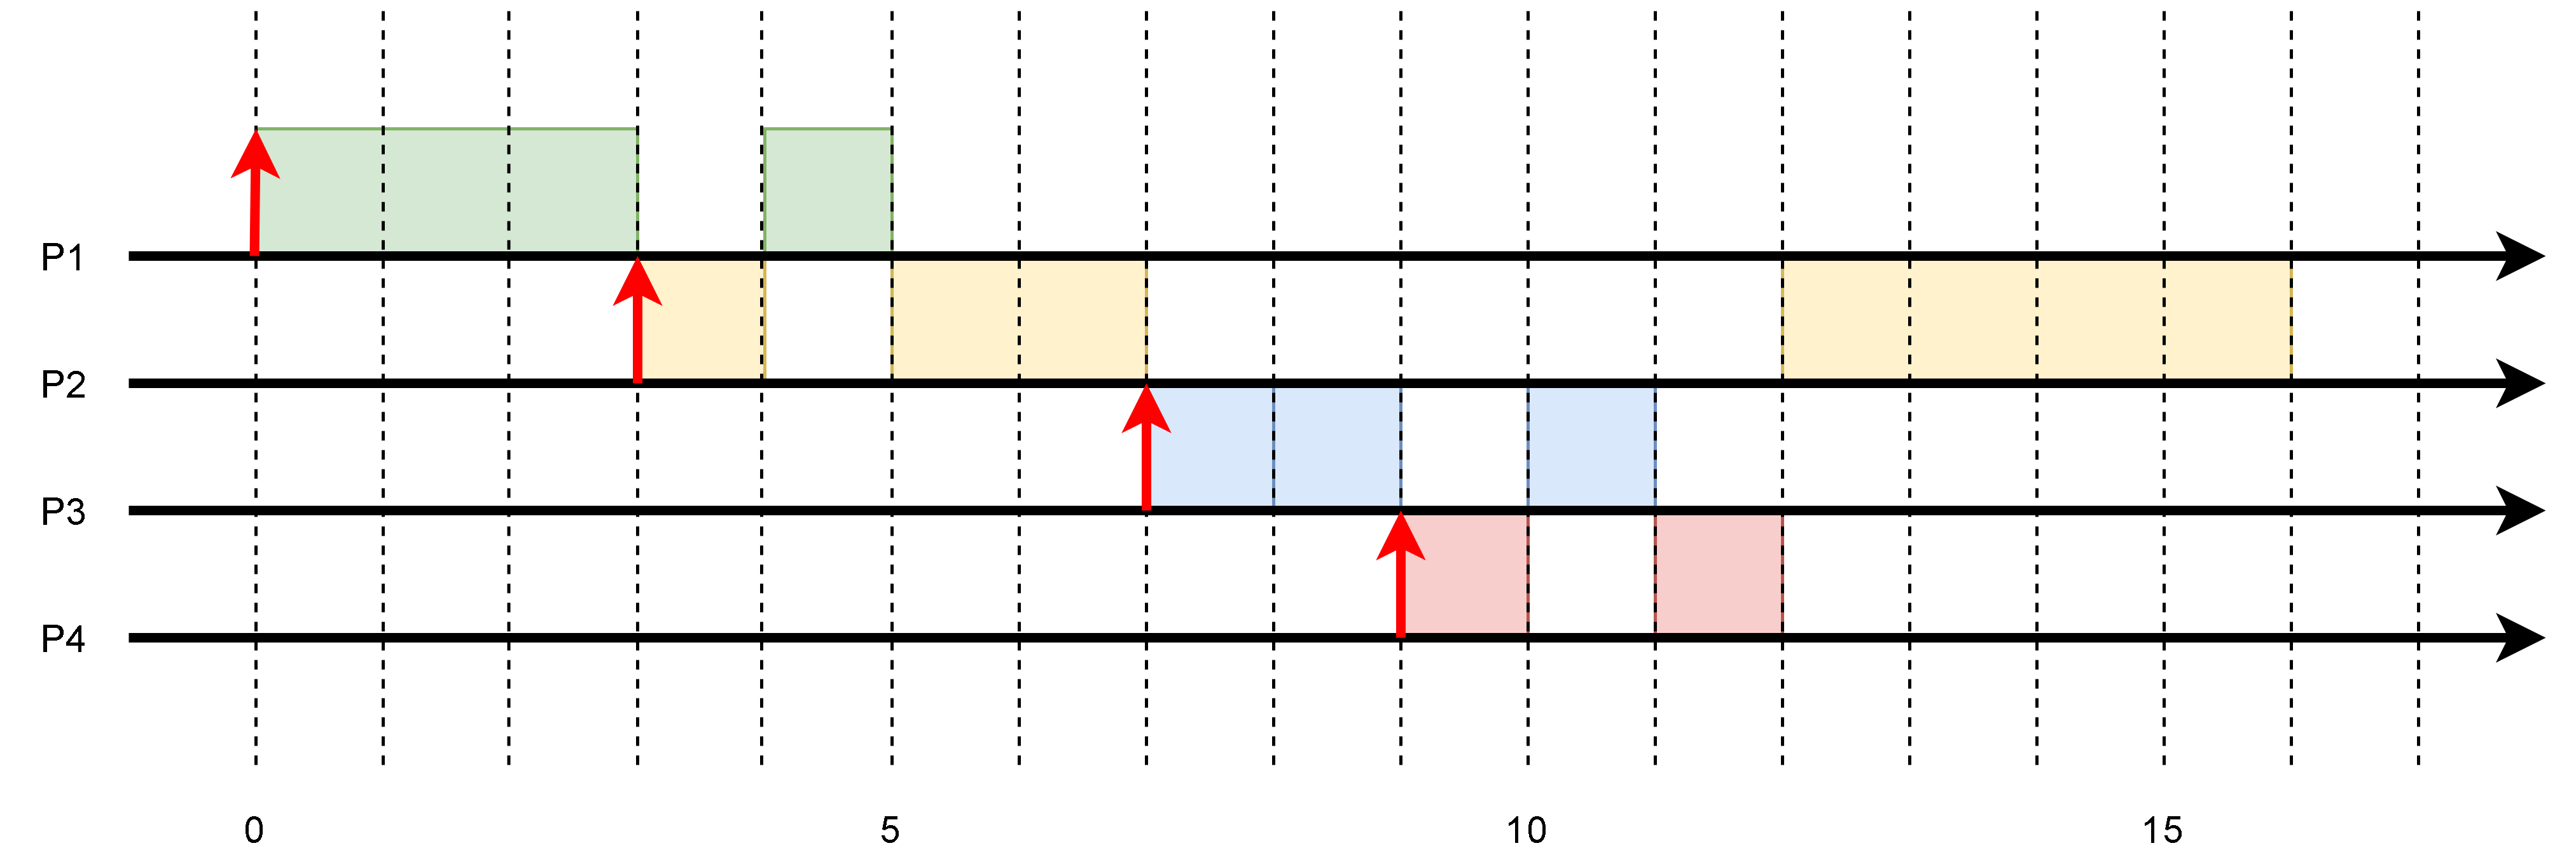
\includegraphics[width=\linewidth]{img/RRP}

\subsubsection{SJF sans priorités (et aussi avec dans ce cas particulier)}
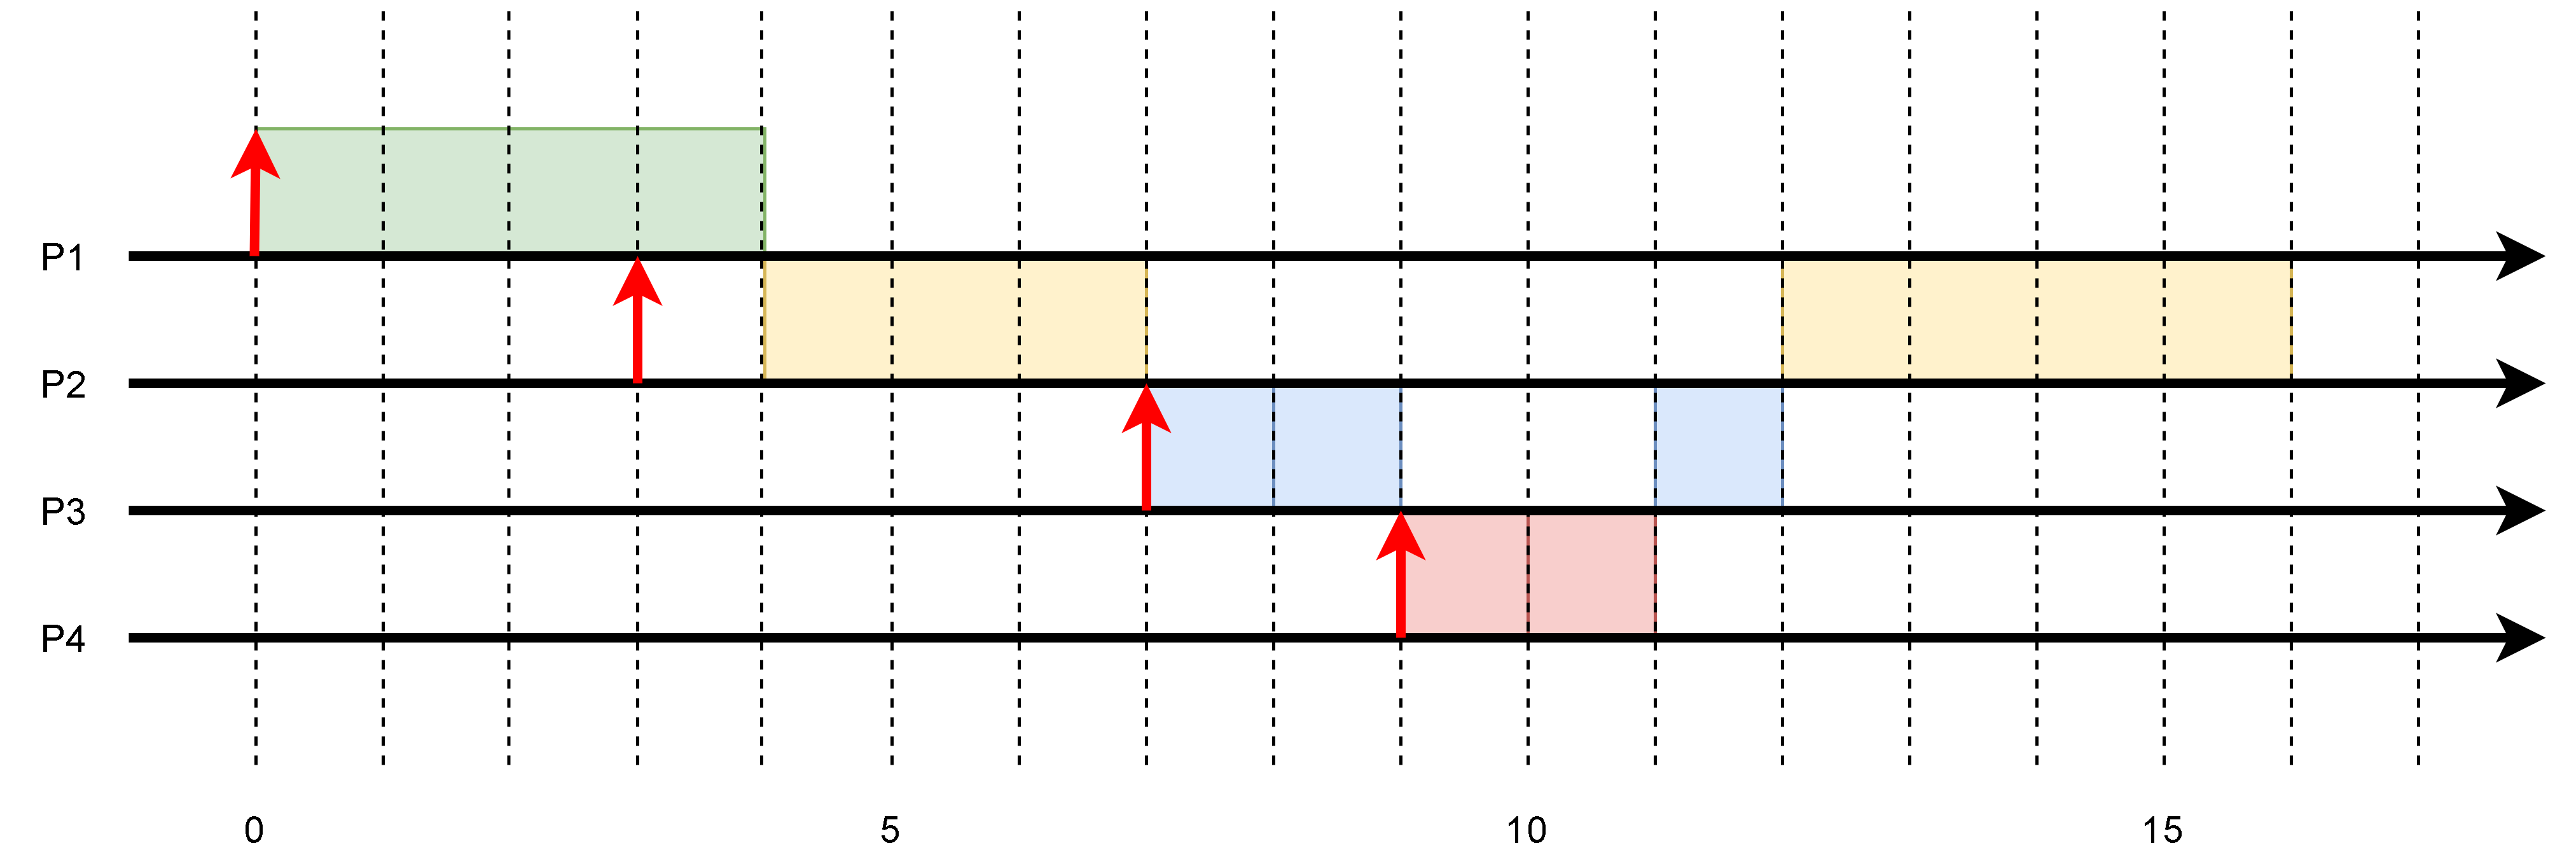
\includegraphics[width=\linewidth]{img/SJF}





\section{L'interblocage}
\subsection{Processus et ressources}
En réalité les algorithmes d'ordonnancement utilisés par les OS actuels font que  l'exécution concurrente des processus est \textit{non déterministe} : l'utilisateur de l'OS ne peut pas prédire quel processus sera exécuté à chaque instant.\\

Or les processus utilisent des \textit{ressources}, et bien souvent celles-ci sont utilisables \textit{de manière exclusive}.\\

Cela veut dire que lorsqu'un processus acquiert l'accès à une ressource, les autres processus ne peuvent y accéder avant que ledit processus n'ait libéré la ressource.

\subsection{Interblocage}
On dit qu'il y a \textit{interblocage} lorsque des processus concurrents s'attendent mutuellement.\\

Dans un article de 1971, Edward Coffman a établi les conditions d'un interblocage, qui portent désormais son nom?
\begin{propriete}[ : conditions de Coffman]
    \begin{itemize}
        \item 	Au moins une ressource doit être conservée par un processus en mode exclusif.
        \item 	Un processus doit conserver une ressource et en demander une autre.
        \item	Une ressource ne peut être libérée que par le processus qui la détient.
        \item 	\textit{Attente circulaire} : Chaque processus doit attendre la libération d'une ressource détenue par un autre qui fait de même.
    \end{itemize}        
\end{propriete}
Dans le cadre de ce chapitre, la condition \textbf{3.} est toujours vérifiée.

\subsection{Exemple Minimaliste}
\begin{itemize}

\item On considère 2 processus P1 et P2 et 2 ressources R1 et R2 \begin{center}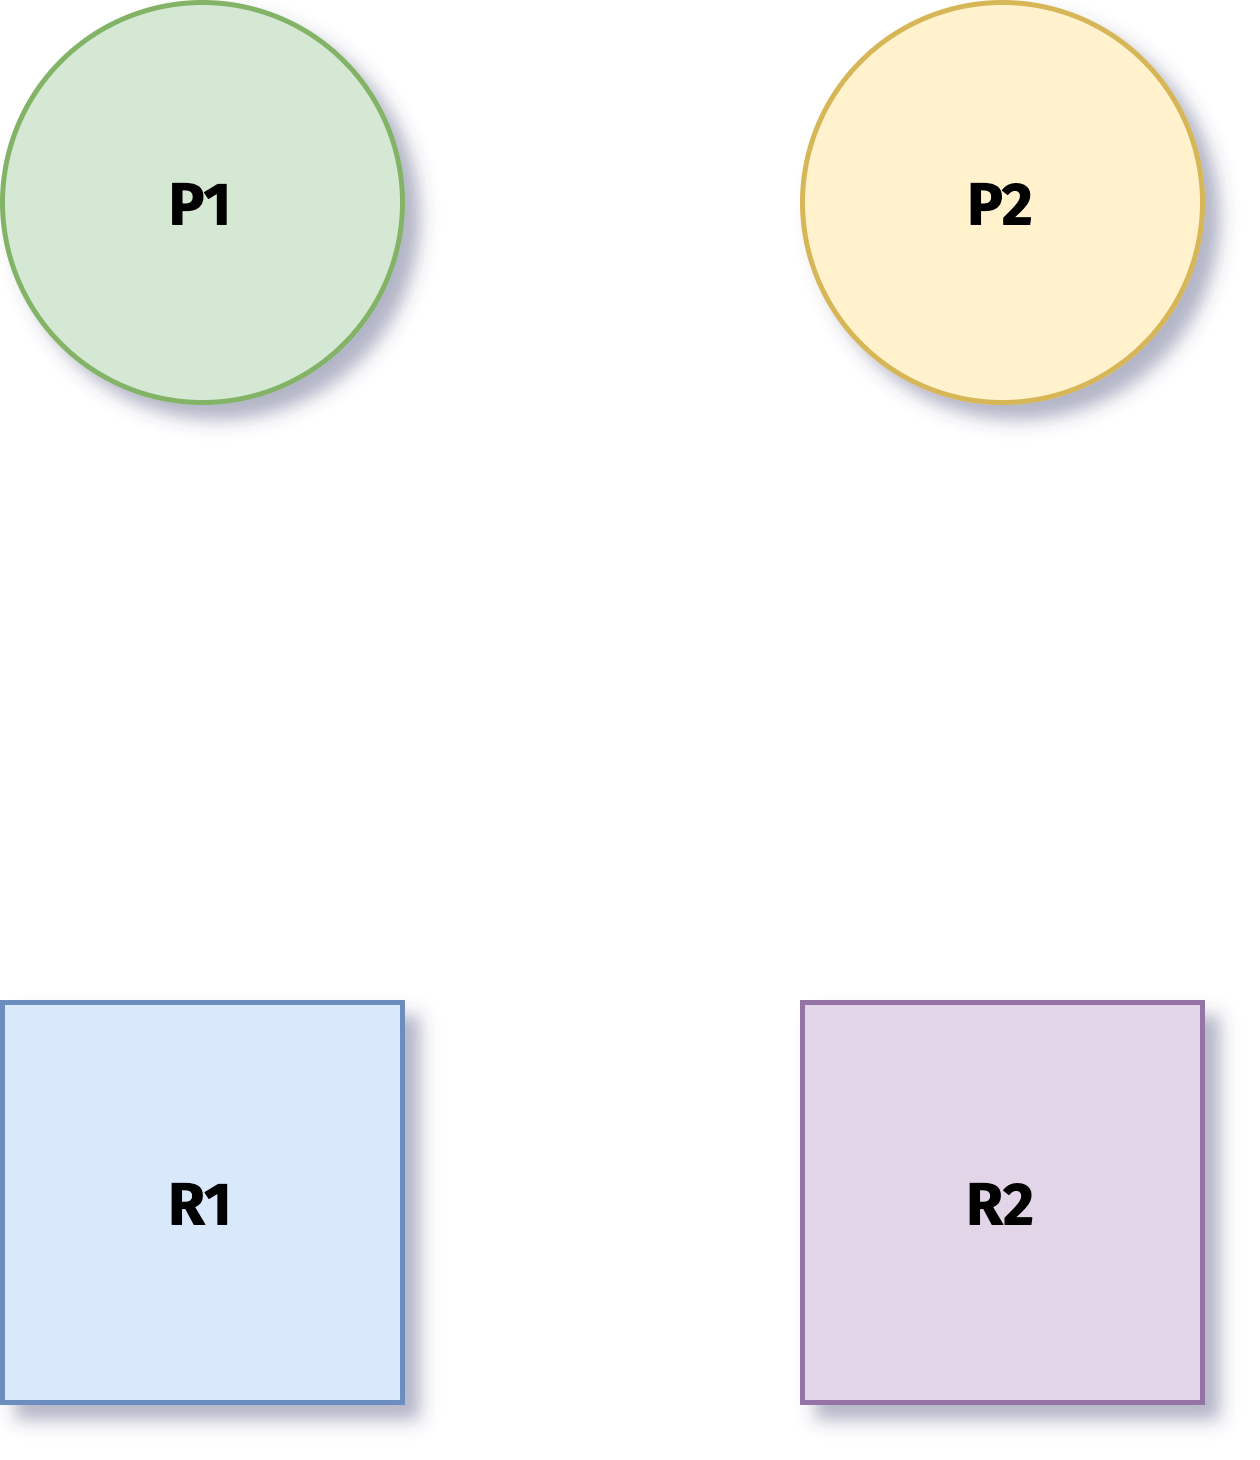
\includegraphics[width=0.2\textwidth]{img/inter1}\end{center}

\item 	P1 demande et obtient l'accès à R1 \begin{center}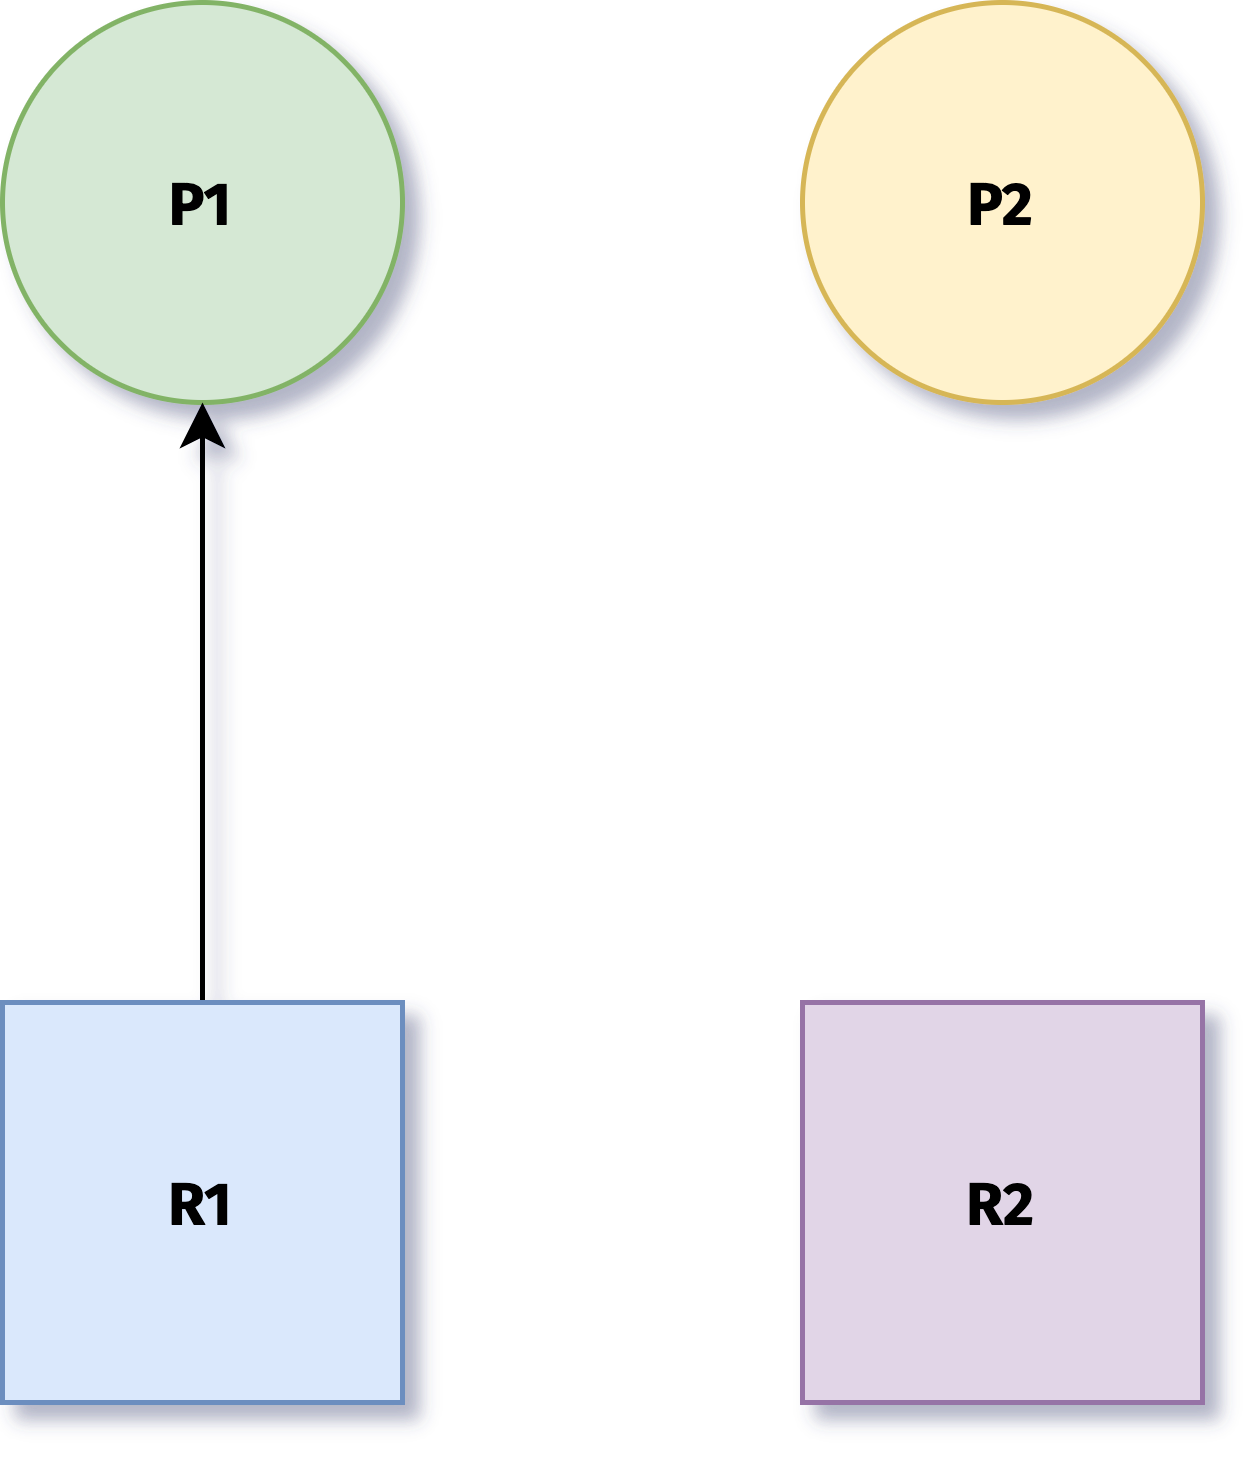
\includegraphics[width=0.2\textwidth]{img/inter2}\end{center}
\item 	P2 demande et obtient l'accès à R2\begin{center}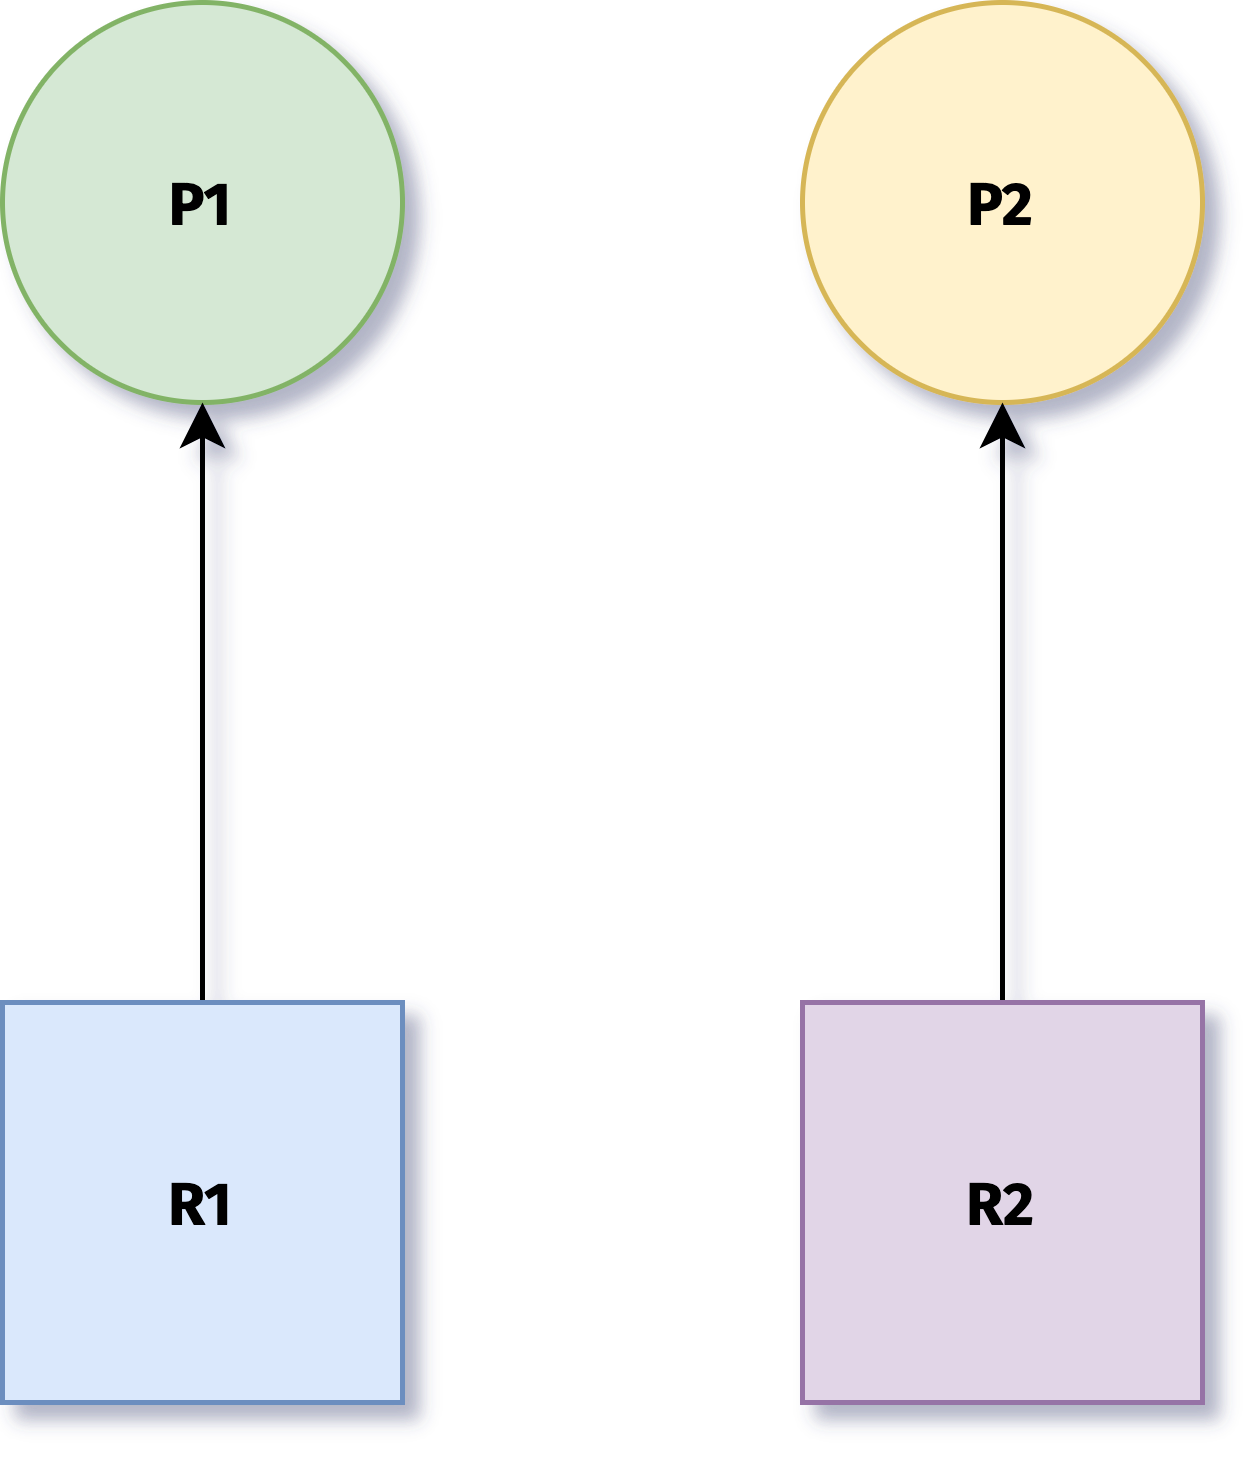
\includegraphics[width=0.2\textwidth]{img/inter3}\end{center}
\item 	P1 demande sans l'obtenir l'accès à R2\begin{center}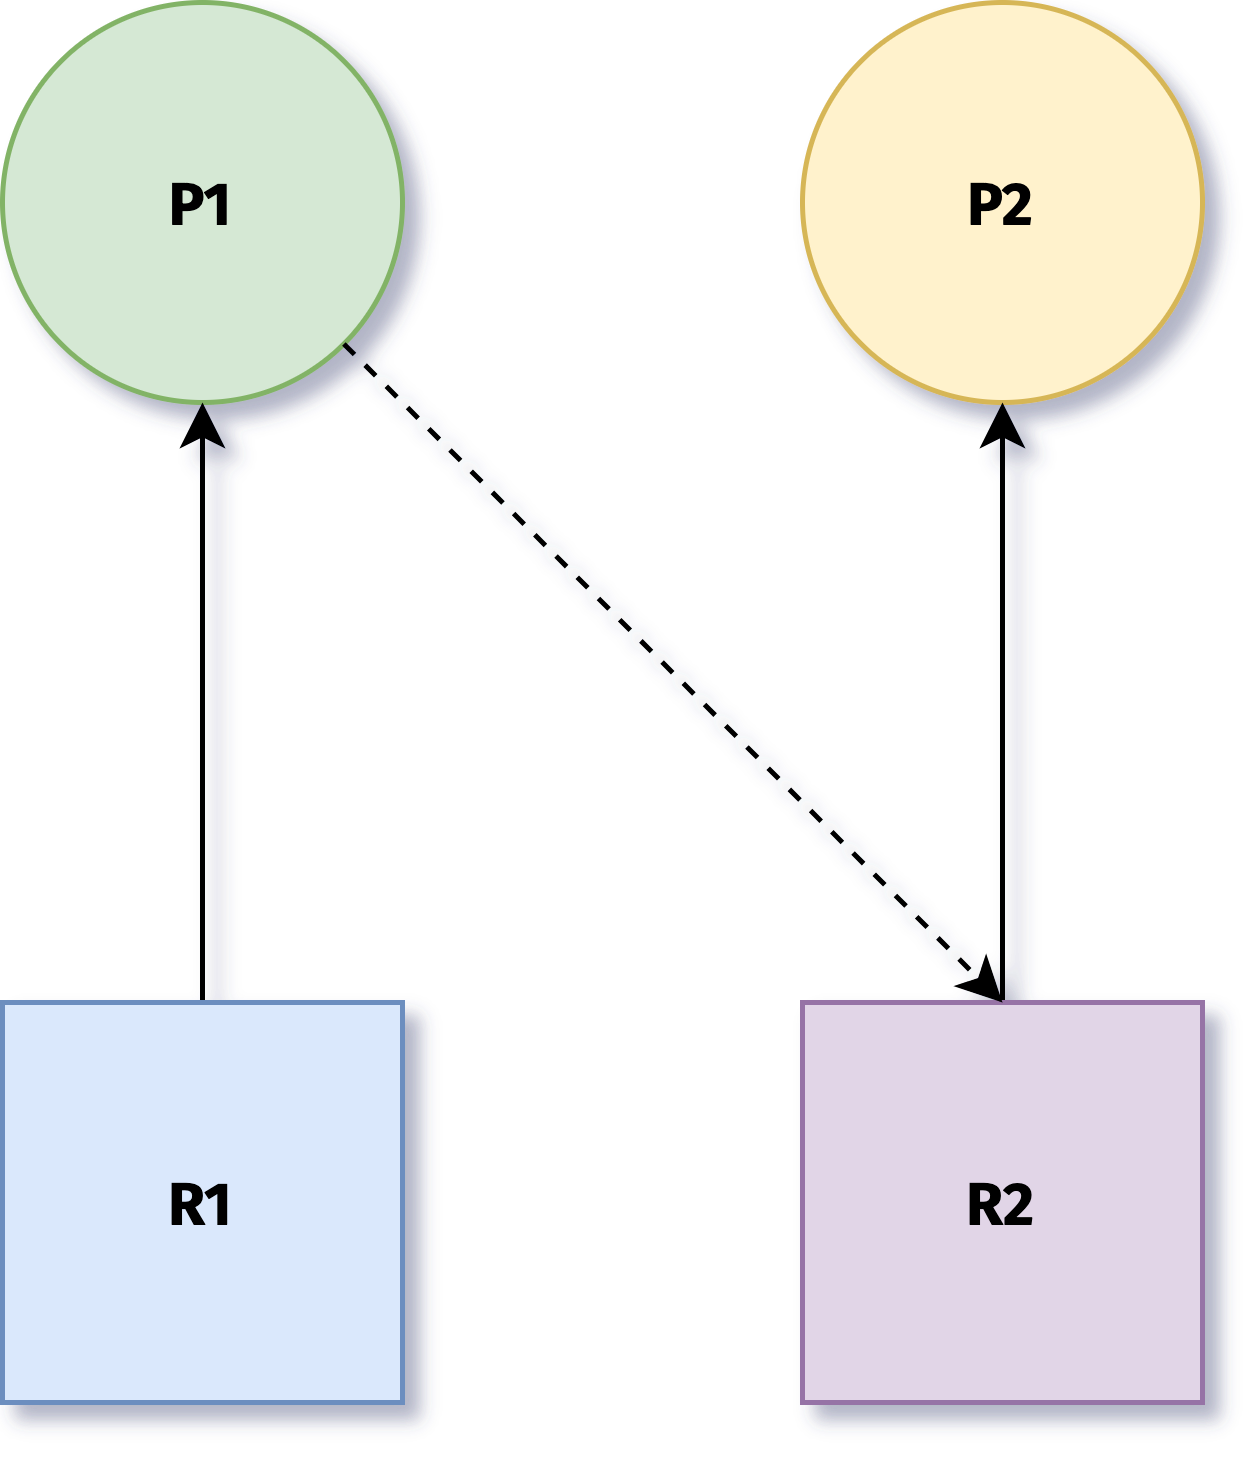
\includegraphics[width=0.2\textwidth]{img/inter4}\end{center}
\item 	P1 attend, P2 demande sans l'obtenir l'accès à R1\begin{center}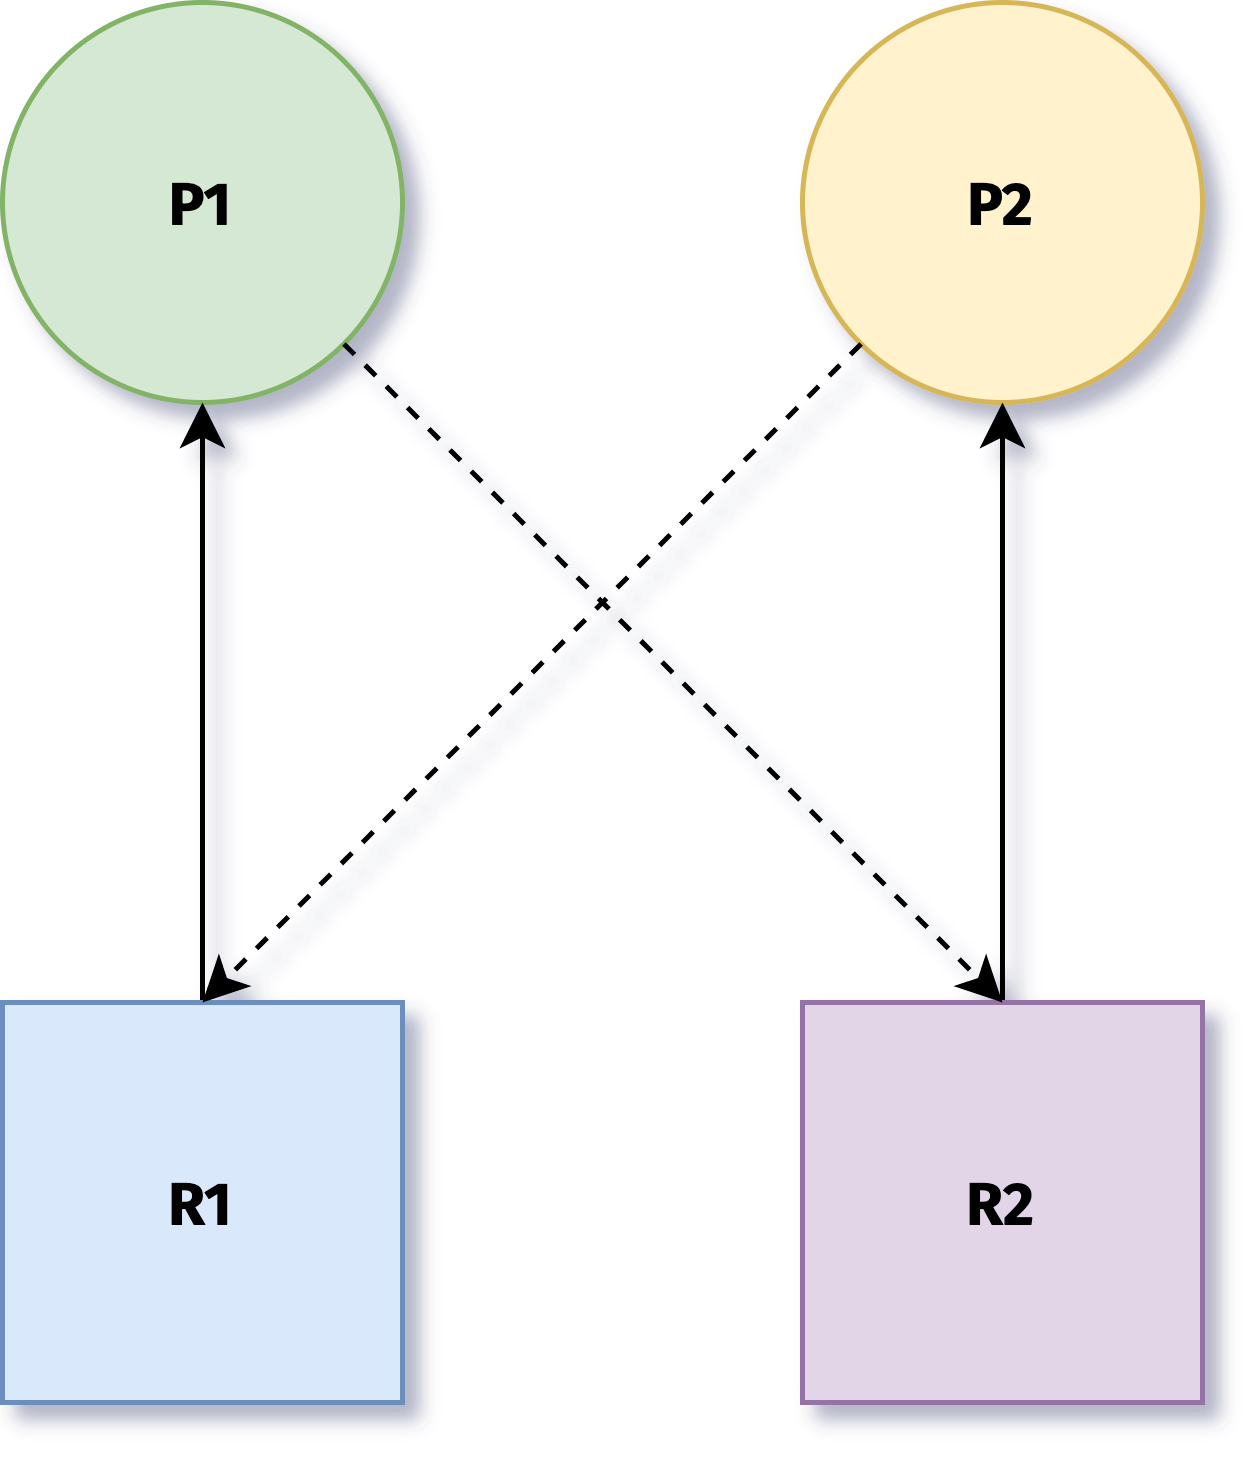
\includegraphics[width=0.2\textwidth]{img/inter5}\end{center}
\item 	P1 attend que P2 libère R2, qui attend que P1 libère R1 : li y a interblocage.
\end{itemize}



\subsection{Solutions à l'interblocage}
\begin{itemize}
	\item 	\textbf{Ne rien faire :} laisser l'utilisateur gérer lui-même le problème (à l'aide de \mintinline{bash}{kill} sous \textsc{linux} ou CTRL+ALT+SUPPR pour lancer le gestionnaire des tâches sous \textsc{Windows}).
	\item 	\textbf{Détecter :}  l'ordonnanceur suit l'allocation des ressources et l'état des processus et redémarre un ou plusieurs d'entre eux si besoin.
    \item \textbf{\'Eviter :} des algorithmes/recettes sont mis en œuvre pour supprimer une des 4 conditions de Coffman nécessaires à la survenue de l'interblocage.
\end{itemize}
\end{document}